%======================================================================
%  UPES  |  School of Computer Science  |  Mid-Sem Assignment Report
%  Template for Applied Machine Learning (CSAI2017P) and
%  Design and Analysis of Algorithms (CSEG3053)
%
%  HOW TO USE
%  1. Overleaf -> New Project -> Upload Project -> choose this .zip.
%     (Or: New Project -> Blank, paste this file, and upload references.bib.)
%  2. Fill in the details in the "YOUR DETAILS" block below.
%  3. Replace every section's placeholder text with your own writing.
%  4. The blue "Guidance" boxes tell you what each section needs.
%     When you are finished, change \showguidancetrue to
%     \showguidancefalse and they will disappear from the PDF.
%======================================================================
\documentclass[11pt,a4paper]{article}
\usepackage{float}

%---------------- Packages ----------------
\usepackage[margin=2.3cm]{geometry}
\usepackage[T1]{fontenc}
\usepackage{amsmath,amssymb}
\usepackage{graphicx}
\usepackage{float}
\usepackage{subcaption}
\usepackage{booktabs}
\usepackage{xcolor}
\usepackage{tikz}
\usetikzlibrary{arrows.meta,positioning,shapes.geometric}
\usepackage{pgfplots}
\pgfplotsset{compat=1.18}
\usepackage[ruled,vlined,linesnumbered]{algorithm2e}
\usepackage{listings}
\usepackage[most]{tcolorbox}
\usepackage{qrcode}
\usepackage{fancyhdr}
\usepackage[hidelinks]{hyperref}

\definecolor{upesnavy}{HTML}{1F3864}
\definecolor{guide}{HTML}{EAF1FB}
\definecolor{codebg}{HTML}{F7F7F7}

%================ YOUR DETAILS (edit these) ================
\newcommand{\studentname}{Adit Kishor Nautiyal}
\newcommand{\sapid}{590024518}
\newcommand{\batch}{B15}                          % B15, B16, B17, B18, B21 or B22
\newcommand{\course}{Applied Machine Learning (CSAI2017P)}
% \newcommand{\course}{Design and Analysis of Algorithms (CSEG3053)}
\newcommand{\topic}{AdaGrad (Adaptive Gradient Algorithm)}
\newcommand{\animationlink}{https://github.com/your-username/adagrad-visualizer}
\newcommand{\submissiondate}{\today}
%============================================================

\newif\ifshowguidance
\showguidancetrue   % change to \showguidancefalse before final submission

\newtcolorbox{guidancebox}{colback=guide,colframe=upesnavy!60,
  fonttitle=\bfseries\small,title=Guidance (delete or hide before submitting),
  fontupper=\small,boxrule=0.5pt,arc=2pt}
% Shows your screenshot if the file exists, otherwise a grey placeholder box,
% so the template compiles even before you add images.
\newcommand{\frameimg}[1]{\IfFileExists{#1}{\includegraphics[width=\linewidth]{#1}}%
  {\fbox{\parbox[c][0.7\linewidth][c]{0.92\linewidth}{\centering\small\color{gray}add\\\texttt{#1}}}}}
\newcommand{\guidance}[1]{\ifshowguidance\begin{guidancebox}#1\end{guidancebox}\fi}

\newtcolorbox{keyidea}{colback=upesnavy!4,colframe=upesnavy,
  fonttitle=\bfseries,title=Key Idea,boxrule=0.6pt,arc=2pt}

\lstset{basicstyle=\ttfamily\small,backgroundcolor=\color{codebg},
  frame=single,rulecolor=\color{gray!40},breaklines=true,
  numbers=left,numberstyle=\tiny\color{gray},keywordstyle=\color{upesnavy}\bfseries,
  commentstyle=\color{gray}\itshape,showstringspaces=false}

\pagestyle{fancy}\fancyhf{}
\lhead{\small\textcolor{upesnavy}{\topic}}
\rhead{\small\studentname\ (\sapid)}
\cfoot{\small\thepage}
\setlength{\headheight}{14pt}

\begin{document}

%======================== TITLE PAGE ========================
\begin{titlepage}
\centering
{\large\textsc{UPES, Dehradun}\par}
{\normalsize School of Computer Science $\cdot$ Artificial Intelligence Cluster\par}
\vspace{2.2cm}
{\color{upesnavy}\rule{\linewidth}{1.2pt}\par}
\vspace{0.6cm}
{\Huge\bfseries\color{upesnavy}\topic\par}
\vspace{0.4cm}
{\Large Mid-Semester Assignment Report\par}
\vspace{0.6cm}
{\color{upesnavy}\rule{\linewidth}{1.2pt}\par}
\vspace{2cm}
\begin{tabular}{rl}
\textbf{Course:}          & \course \\[3pt]
\textbf{Student:}         & \studentname \\[3pt]
\textbf{SAP ID:}          & \sapid \\[3pt]
\textbf{Batch:}           & \batch \\[3pt]
\textbf{Semester:}        & III (Aug--Dec 2026) \\[3pt]
\textbf{Submitted to:}    & Kunwar Siddharth, Assistant Professor \\[3pt]
\textbf{Date:}            & \submissiondate \\
\end{tabular}
\vfill
\begin{tabular}{c}
\qrcode[height=3cm]{https://github.com/Adit1N/ML-Project-Adagrad-}\\[4pt]
\small Scan to open the animation / code
\end{tabular}
\end{titlepage}

%======================== ABSTRACT ========================
\begin{abstract}
AdaGrad (Adaptive Gradient Algorithm) is a first-order optimization method designed to adjust learning rates independently for individual model parameters. Unlike conventional gradient descent, which typically applies a common learning rate, AdaGrad accumulates the squared gradients of each parameter and uses this history to scale subsequent updates. This mechanism can be particularly useful in learning problems involving sparse features or substantially different gradient magnitudes. This project investigates AdaGrad using a two-dimensional quadratic objective function with unequal curvature along its coordinate axes. A Python-based interactive visualization is developed to illustrate the parameter trajectory, objective value, accumulated squared gradients, and coordinate-wise effective learning rates across successive iterations. The experiment is intended to examine how gradient history influences update magnitudes and optimization behaviour. A key limitation of AdaGrad is that its accumulated squared gradients never decrease, causing effective learning rates to shrink over time. Consequently, parameter updates may become excessively small, potentially slowing further optimization progress. The analysis evaluates these characteristics using the numerical trace and graphical outputs generated by the implementation.
\end{abstract}

\tableofcontents
\newpage

%======================== 1 INTRODUCTION ========================
\section{Introduction}

Optimization is a fundamental process in machine learning that involves finding model parameters that minimize an objective function, typically representing prediction error. Gradient-based methods perform this optimization iteratively by adjusting parameters according to the gradients of the objective function. However, selecting an appropriate learning rate is challenging when different parameters have gradients with substantially different magnitudes. A single global learning rate may produce excessively large updates for some parameters while causing slow progress for others.

AdaGrad (Adaptive Gradient Algorithm) addresses this limitation by accumulating the squared gradients independently for each parameter and using these accumulated values to scale subsequent updates. Consequently, parameters with larger accumulated gradient magnitudes receive smaller effective learning rates, while parameters with smaller accumulated values can retain comparatively larger learning rates. This property can be beneficial in sparse-feature applications such as text classification, where certain words appear frequently while others occur infrequently but may provide useful classification information. AdaGrad was developed as an adaptive subgradient method for online learning and stochastic optimization \cite{duchi2011}.

This project investigates AdaGrad using a two-dimensional convex quadratic objective function with different curvature along its coordinate axes. A Python-based visualization is used to examine the optimization trajectory, changes in the objective value, accumulated squared gradients, and coordinate-wise effective learning rates. The experiment aims to illustrate how gradient history influences parameter updates and to investigate a key limitation of AdaGrad: accumulated squared gradients never decrease, so effective learning rates may become progressively smaller and eventually hinder further optimization progress \cite{mcmahan2017}.

%======================== 2 INTUITION ========================
\section{Intuition and Core Idea}

The main idea behind AdaGrad is that different model parameters may require different learning rates. During model training, the gradient indicates how the loss function changes with respect to each parameter. A large gradient suggests a strong local change in the loss, whereas a small gradient indicates a weaker local change. Using the same learning rate for every parameter may therefore produce inefficient updates when their gradient magnitudes differ considerably.

AdaGrad addresses this problem by maintaining a separate history of squared gradients for each parameter. Whenever a gradient is calculated, its square is added to the corresponding accumulated value. Parameters that repeatedly receive large gradients build up larger accumulators and consequently receive smaller effective learning rates. Parameters with smaller accumulated squared gradients retain comparatively larger effective learning rates. This mechanism allows the optimizer to adapt its updates according to the gradient history of individual parameters \cite{duchi2011}.

Figure~\ref{fig:adagrad-flow}  illustrates the sequence of operations performed during an AdaGrad iteration. First, the current parameter values are used to calculate the gradient of the objective function. Next, the squared gradient components are added to their respective accumulators. The accumulated values are then used to scale the gradient, producing coordinate-wise adaptive updates. Finally, the parameters are updated, and the process repeats until the chosen stopping condition is reached.

An important characteristic of AdaGrad is that its accumulated squared gradients never decrease. Consequently, the effective learning rates are non-increasing over time. Although this can be beneficial for adapting updates to different gradient scales, it may also cause learning rates to become too small during prolonged optimization.

\begin{keyidea}
AdaGrad accumulates the square of each coordinate's gradients and divides the
current gradient by the square root of that coordinate's accumulated history.
Coordinates with larger accumulated gradients therefore receive smaller
effective step sizes.
\end{keyidea}

%---- Figure 1: AdaGrad update flow ----
\begin{figure}[h]
\centering
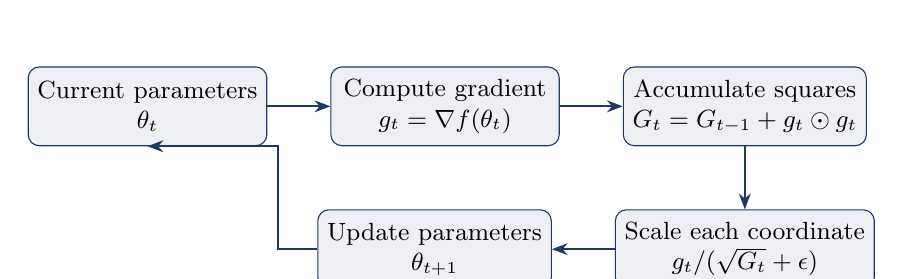
\begin{tikzpicture}[
  node distance=8mm and 8mm,
  block/.style={draw=upesnavy,rounded corners,fill=upesnavy!8,
                align=center,minimum width=29mm,minimum height=10mm,font=\small},
  arrow/.style={-{Stealth[length=2mm]},thick,draw=upesnavy}]
\node[block] (theta) {Current parameters\\$\theta_t$};
\node[block,right=of theta] (grad) {Compute gradient\\$g_t=\nabla f(\theta_t)$};
\node[block,right=of grad] (acc) {Accumulate squares\\$G_t=G_{t-1}+g_t\odot g_t$};
\node[block,below=of acc] (scale) {Scale each coordinate\\$g_t/(\sqrt{G_t}+\epsilon)$};
\node[block,left=of scale] (update) {Update parameters\\$\theta_{t+1}$};
\draw[arrow] (theta) -- (grad);
\draw[arrow] (grad) -- (acc);
\draw[arrow] (acc) -- (scale);
\draw[arrow] (scale) -- (update);
\draw[arrow] (update.west) -- ++(-5mm,0) |- (theta.south);
\end{tikzpicture}
\caption{AdaGrad iteration: compute the gradient, accumulate its coordinate-wise square, scale the update, and repeat.}
\label{fig:adagrad-flow}
\end{figure}

%======================== 3 MATHEMATICS ========================
\section{Mathematical Formulation}

Let $\theta_t\in\mathbb{R}^d$ be the parameter vector and
$g_t=\nabla f(\theta_t)$ the gradient at iteration $t$. AdaGrad stores
the cumulative squared-gradient vector
\begin{equation}
G_t=G_{t-1}+g_t\odot g_t,\qquad G_{-1}=\mathbf{0},
\label{eq:accumulator}
\end{equation}
where $\odot$ denotes element-wise multiplication. The coordinate-wise
effective learning rate is
\begin{equation}
\eta_{t,i}^{\mathrm{eff}}=
\frac{\eta}{\sqrt{G_{t,i}}+\epsilon},
\label{eq:effective-lr}
\end{equation}
and the parameter update is
\begin{equation}
\theta_{t+1}=\theta_t-
\eta\,\frac{g_t}{\sqrt{G_t}+\epsilon}.
\label{eq:update}
\end{equation}
Square roots and divisions in Equation~\ref{eq:update} are applied
element-wise. Here $\eta>0$ is the base learning rate and $\epsilon>0$
is a small stability constant. Implementations sometimes place $\epsilon$
inside the square root; this report uses the convention shown above.

For the visualization, use the objective
\begin{equation}
f(x,y)=\frac{1}{2}(x^2+10y^2),\qquad
\nabla f(x,y)=\begin{bmatrix}x\\10y\end{bmatrix}.
\label{eq:objective}
\end{equation}
Its Hessian is $\nabla^2 f=\operatorname{diag}(1,10)$, which is positive
definite. Thus the objective is strictly convex and has the unique minimizer
$(x^\star,y^\star)=(0,0)$. The unequal curvature makes the gradient scales
different across the two coordinates, making coordinate-wise adaptation
visible.

% Add your own generated plot here. Keep the filename consistent with the
% actual figure uploaded to Overleaf.
\begin{figure}[H]
    \centering
    \includegraphics[width=0.65\linewidth]{figures/figure1_trajectory.png}
    \caption{AdaGrad trajectory over the contour lines of the quadratic objective function.}
    \label{fig:trajectory}
\end{figure}

%======================== 4 ALGORITHM ========================
\section{Algorithm / Procedure}

\begin{algorithm}[h]
\caption{AdaGrad for minimizing a differentiable objective}
\KwIn{Objective $f$, gradient $\nabla f$, initial parameters $\theta_0$,
learning rate $\eta$, stability constant $\epsilon$, iteration count $T$}
\KwOut{Updated parameters $\theta_T$}
$G \leftarrow \mathbf{0}$; $\theta \leftarrow \theta_0$\;
\For{$t \leftarrow 0$ \KwTo $T-1$}{
  $g \leftarrow \nabla f(\theta)$\;
  $G \leftarrow G + g \odot g$\;
  $\theta \leftarrow \theta - \eta\,g/(\sqrt{G}+\epsilon)$\;
}
\Return $\theta$\;
\end{algorithm}

\textbf{Implementation convention.} The code updates the accumulator with the
current gradient before computing the parameter step. For a dense vector of
$d$ parameters, the accumulator and update require $O(d)$ operations and
$O(d)$ extra memory per iteration, excluding gradient-computation cost.

Short implementation excerpt (the full interactive program is in the linked repository):
\begin{lstlisting}[language=Python]
gradient = grad(theta)
accumulator += gradient ** 2
effective_lr = eta / (np.sqrt(accumulator) + epsilon)
theta = theta - effective_lr * gradient
\end{lstlisting}

%======================== 5 WORKED EXAMPLE ========================
\section{Worked Example (Step by Step)}

Consider the objective function $f(w)=w^2$, with initial parameter
$w_0=2$ and learning rate $\eta=0.1$. Its gradient is
\[
g_t = \frac{df}{dw}=2w_t.
\]

The cumulative squared-gradient accumulator is updated as
\[
G_t = G_{t-1}+g_t^2,\qquad G_{-1}=0,
\]
and the parameter update is
\[
w_{t+1}=w_t-\eta\frac{g_t}{\sqrt{G_t}}.
\]

For simplicity, $\epsilon$ is omitted in the hand calculations.
The Python implementation includes $\epsilon$ in the denominator
for numerical stability.

At iteration $t=0$, the gradient is $g_0=2(2)=4$ and the
accumulator becomes $G_0=0+4^2=16$. Therefore,
\[
w_1=2-\frac{0.1(4)}{\sqrt{16}}=1.9.
\]

At each subsequent iteration, the new squared gradient is added
to the existing accumulator. The updated accumulator determines
the effective learning rate $\eta_t^{\mathrm{eff}}$ and the
parameter step $\Delta w_t$:
\[
\eta_t^{\mathrm{eff}}=\frac{\eta}{\sqrt{G_t}},
\qquad
\Delta w_t=\eta_t^{\mathrm{eff}}g_t.
\]

\begin{table}[htbp]
\centering
\small
\begin{tabular}{@{}rrrrrr@{}}
\toprule
$t$ & $w_t$ & $g_t$ & $G_t$ &
$\eta_t^{\mathrm{eff}}$ & $w_{t+1}$ \\
\midrule
0 & 2.0000 & 4.0000 & 16.0000 & 0.0250 & 1.9000 \\
1 & 1.9000 & 3.8000 & 30.4400 & 0.0181 & 1.8311 \\
2 & 1.8311 & 3.6623 & 43.8521 & 0.0151 & 1.7758 \\
3 & 1.7758 & 3.5516 & 56.4663 & 0.0133 & 1.7286 \\
\bottomrule
\end{tabular}
\caption{Hand calculation of AdaGrad updates for $f(w)=w^2$
with $\eta=0.1$ and $\epsilon$ omitted. Values are rounded.}
\label{tab:adagrad-worked}
\end{table}

The example illustrates that the accumulated squared gradients
increase at each iteration, causing the effective learning rate
to decrease. Consequently, the parameter approaches the minimum
at $w=0$ through progressively smaller updates for these
iterations. The example demonstrates the update mechanism but
does not, by itself, establish convergence for all objective
functions.


[STUDENT: Add a paragraph interpreting how the accumulated sum changes and
how this affects the effective learning rate. Explain why the exact application
trace can differ slightly because it includes epsilon.]

%======================== 6 ANIMATION ========================
\section{Animation / Software Demonstration}

The AdaGrad visualizer was developed using Python, NumPy,
Matplotlib, and Streamlit. It demonstrates the optimization
process on the two-dimensional quadratic objective
\[
f(x,y)=\frac{1}{2}(x^2+10y^2).
\]

The application provides controls for changing the initial
values of $x$ and $y$, the base learning rate $\eta$,
the numerical-stability constant $\epsilon$, and the total
number of iterations. An iteration slider allows the user
to inspect intermediate optimization states.

The visualization displays the parameter trajectory over
the loss contours, the objective value across iterations,
the coordinate-wise effective learning rates, and a
numerical trace containing gradients, accumulated squared
gradients, and parameter updates.

\paragraph{How to Run.}
Install the dependencies listed in \texttt{requirements.txt }. Then execute
\texttt{streamlit run app.py} from the animation directory.
The application opens in a web browser.

\paragraph{Source Code.}
\url{https://github.com/Adit1N?tab=repositories}.

\paragraph{Key Frames.}
Figures~\ref{fig:frame1}--\ref{fig:frame4} show four
states captured from the running application. They
illustrate the initial configuration, an early update,
an intermediate iteration, and the final displayed state.

% Replace these four filenames with your actual screenshots.
\begin{figure}[H]
    \centering
    \includegraphics[width=0.75\linewidth]{figures/frame1.png}
    \caption{Initial parameter configuration.}
    \label{fig:frame1}
\end{figure}

\begin{figure}[H]
    \centering
    \includegraphics[width=0.75\linewidth]{figures/frame2.png}
    \caption{Early AdaGrad parameter update.}
    \label{fig:frame2}
\end{figure}

\begin{figure}[H]
    \centering
    \includegraphics[width=0.75\linewidth]{figures/frame3.png}
    \caption{Intermediate optimization state.}
    \label{fig:frame3}
\end{figure}

\begin{figure}[H]
    \centering
    \includegraphics[width=0.75\linewidth]{figures/frame4.png}
    \caption{Final displayed optimization state.}
    \label{fig:frame4}
\end{figure}

\textbf{Tool used:} Python, NumPy, Matplotlib, and Streamlit.\\
\textbf{Link:} \url{\animationlink}\\
\textbf{How to run:} In the \texttt{animation} folder, run
\texttt{python -m pip install -r requirements.txt}, then
\texttt{streamlit run app.py}.\\
\textbf{What the viewer can change:} initial $x$ and $y$, base learning rate,
epsilon, total iterations, and the iteration displayed. The app plots the
parameter trajectory, loss curve, effective learning rates, and numerical trace.

%======================== 7 ANALYSIS ========================
\section{Analysis}

\subsection{Assumptions}
The experiment minimizes the differentiable objective
$f(x,y)=\frac{1}{2}(x^2+10y^2)$ using its analytical gradient.
The initial parameters are $x=4$ and $y=3$, the base learning rate
is $\eta=0.30$, and the numerical-stability constant is
$\epsilon=10^{-6}$. The accumulator starts at zero. The experiment
uses a deterministic gradient rather than randomly sampled
mini-batches; therefore, it illustrates the adaptive update rule
but does not reproduce every aspect of stochastic training.

For a dense parameter vector of dimension $d$, maintaining the accumulator
and applying the parameter update cost $O(d)$ time and $O(d)$ additional memory
per iteration. The full iteration also includes the cost of evaluating the
gradient, which can dominate for large models.

\begin{table}[h]
\centering
\begin{tabular}{@{}lll@{}}
\toprule
\textbf{Criterion} & \textbf{AdaGrad} & \textbf{Plain SGD}\\
\midrule
Learning rate & Coordinate-wise adaptive & Usually global scalar\\
Extra state & $O(d)$ accumulator & Often $O(1)$ optimizer state\\
Sparse gradients & Can be useful & May need careful tuning\\
Main limitation & Effective rates can become tiny & Sensitive to global rate\\
\bottomrule
\end{tabular}
\caption{Qualitative comparison of AdaGrad and plain SGD.}
\label{tab:comparison}
\end{table}

\textbf{Strengths.} AdaGrad scales each coordinate using its accumulated
gradient history and can be useful when feature frequencies or gradient
magnitudes differ substantially.

\textbf{Limitations.} Since $G_{t,i}$ never decreases, the effective learning
rate for each coordinate is non-increasing under this update convention. It may
become too small for useful progress late in training. Results also depend on
the base learning rate, epsilon, objective, and gradient noise. The visualization
of one convex function is not proof that AdaGrad is optimal for every model.

Experimental Observations

In the animation, the trajectory and loss curve show how the
parameters move toward a lower-loss region. The effective
learning-rate plot illustrates how the update scale changes over
iterations. In this experiment, compare the initial and final
losses and inspect the parameter trajectory. Since the experiment
does not include a separate SGD run, it demonstrates AdaGrad's
behavior but does not establish that it outperforms SGD on this
objective.


%======================== 8 APPLICATIONS ========================
\section{Applications}

\subsection{Natural Language Processing}
AdaGrad is useful in natural language processing (NLP), particularly
for learning word representations and training models with sparse
features. In text classification, a document may activate only a
small subset of the available vocabulary features. AdaGrad adjusts
the learning rate separately for each parameter according to its
accumulated squared gradients, allowing parameters with relatively
infrequent updates to retain larger effective learning rates.
This property makes it suitable for high-dimensional, sparse
learning problems \cite{duchi2011}.

\subsection{Online Learning and Recommendation Systems}
In online learning, models are updated as new user interactions
or data samples arrive. For example, a recommendation system may
update its parameters when a user clicks, rates, or purchases an
item. AdaGrad adapts parameter-wise update sizes using the history
of observed gradients. This can be useful when user preferences
and feature frequencies vary significantly over time. However,
because the accumulated squared gradients continually increase,
the effective learning rates may become too small when the data
distribution changes substantially.

\subsection{Machine Learning with Sparse Features}
AdaGrad can also be applied to classification and prediction tasks
with high-dimensional sparse input features, such as spam detection
and click-through-rate prediction. In spam detection, features may
represent individual words or phrases, and many features occur
infrequently. AdaGrad maintains a separate squared-gradient
accumulator for each model parameter and scales subsequent updates
accordingly. This enables different features to receive different
effective learning rates without manually tuning a separate rate
for every parameter \cite{duchi2011}.

\subsection{Summary}
These applications illustrate AdaGrad's main advantage: automatic,
coordinate-wise learning-rate adaptation. 

%======================== 9 CONCLUSION ========================
\section{Conclusion}

AdaGrad is an adaptive optimization algorithm that adjusts the
learning rate of each parameter using the cumulative sum of its
past squared gradients. This allows different parameters to receive
different update sizes during optimization.

In this experiment, AdaGrad was applied to the objective function
$f(x,y)=\frac{1}{2}(x^2+10y^2)$, starting from $(x,y)=(4,3)$
with a base learning rate of $0.30$ and $\epsilon=10^{-6}$.
The trajectory and loss plots were used to observe the optimization
process. One observed result was that the loss decreased from
[initial loss] to [final loss] after 30 iterations.

One limitation of this experiment is that it uses a simple,
deterministic two-variable function rather than a large real-world
machine-learning dataset. Therefore, the results do not establish
how AdaGrad would perform on more complex learning tasks.

A meaningful direction for future work is to compare AdaGrad with
plain stochastic gradient descent using the same objective function,
initial parameters, and controlled learning-rate settings. This
would help evaluate how adaptive learning rates affect convergence
and final loss.

%======================== DECLARATION ========================
\section*{Declaration of AI Tool Use}

\begin{itemize}
    \item \textbf{Tools used:} ChatGPT (OpenAI).

    \item \textbf{What for:} ChatGPT was used to assist with
    understanding the AdaGrad algorithm, explaining mathematical            concepts, help with Python animation code, and providing                       guidance on debugging and interpreting optimization plots.

    \item \textbf{Approximate share of AI-generated content:}
    [15-20]\%.
\end{itemize}

I confirm that I have reviewed the submitted report and animation,
verified the results I present, and taken responsibility for the
final submission. The work has been completed in accordance with
the course's academic integrity requirements.

\vspace{1.5cm}

\noindent
\begin{minipage}{0.48\textwidth}
    \textbf{Signature:}\\[0.3cm]
    \rule{5cm}{0.4pt}
\end{minipage}
\hfill
\begin{minipage}{0.40\textwidth}
    \textbf{Date:}\\[0.3cm]
    \rule{3.5cm}{0.4pt}
\end{minipage}

%======================== REFERENCES ========================
\bibliographystyle{ieeetr}
\bibliography{references}

\end{document}
